\documentclass[10pt]{article}
\usepackage{fancyhdr}
\usepackage[colorlinks=true, linkcolor=blue, urlcolor=blue, citecolor=blue]{hyperref}
\usepackage{dirtree}
\usepackage[margin=0.6in]{geometry}
\usepackage{graphicx}

\title{Angry Birds Game}
\author{Pawan Kumar Meena}
\date{29/04/2025}

\begin{document}

\maketitle
\begin{abstract}
    This report presents the development of a two-player physics-based Angry Birds-style game built using Pygame. The game features a slingshot mechanic, destructible structures, and a selection system allowing players to choose the order of their birds before launching. Core aspects of the project include implementing realistic physics and interactive gameplay.
\end{abstract}

\vspace{1cm}

\begin{center}
    \tableofcontents
\end{center}

\newpage

\section{Introduction}\label{sec:Introduction}
This is two-player game, where you compete with your friend and try to destroy all the opponent's blocks before them and thus winning the game. We have to use different mechanics of the birds to destroy the blocks as quick as possible.

\section{Modules}\label{sec:Modules}
The Modules used in this project are:
\begin{itemize}
    \item \textbf{pygame-ce:} A Python library for writing video games.
    \item \textbf{sys:} Provides access to system-specific parameters and functions
    \item \textbf{math:} Provides access to various mathematical functions
    \item \textbf{random:} Provides access to random number generation
\end{itemize}
For functions like time, I used the pygame library.

\section{Directory Structure}\label{sec:Directory-Structure}
My project directory looks like the following:

\vspace{1cm}
\dirtree{%
    .1 Angry Birds.
    .2 assets.
    .3 animation-explosion.
    .3 audio.
    .3 background-images.
    .3 Birds.
    .3 icons.
    .3 instruction-images.
    .3 object.
    .3 {report\_images}.
    .2 {game\_end.py}.
    .2 {game.py}.
    .2 {loop.py}.
    .2 {main\_menu.py}.
    .2 {settings.py}.
    .2 {teams.py}.
}

\begin{itemize}
    \item \textbf{assets:} This folder contains all the assets used in the game, including images, sounds, and animation frames.
    \item \textbf{game.py:} This is the game file which we'll run to play the game.
    \item \textbf{settings.py:} Contains the size of game screen.
    \item \textbf{game\_end.py, loop.py, main\_menu.py, teams.py} These files contain the game loop, game main menu, end screen design, and teams logic.
\end{itemize}

\vspace{1cm}
\section{Running instructions}\label{sec:Running-instructions}


\subsection{Setting up}\label{subsec:Setting-up}
To run the game, we need python installed and the modules mentioned above installed. I recommend using a virtual environment to avoid any conflicts with other project on your system. You can create a virtual environment using the following command:
\begin{verbatim}
                    python3.X -m venv my_venv           (Replace X with your desired python version)
                    source my_venv/bin/activate         (Linux or Mac)
                    my_venv\Scripts\activate            (Windows)
                    pip install pygame-ce
                \end{verbatim}
After that, you can run the game using the following command in your terminal:
\begin{verbatim}
                    python3 game.py
                \end{verbatim}


\subsection{Game Navigation}\label{subsec:Game Navigation}
\subsubsection{Game intro}
As soon as you hit enter button after writing the previous command, you will start hearing the OG angry birds music, with your screen now displaying the game intro screen.

\begin{figure}[h!]
    \centering
    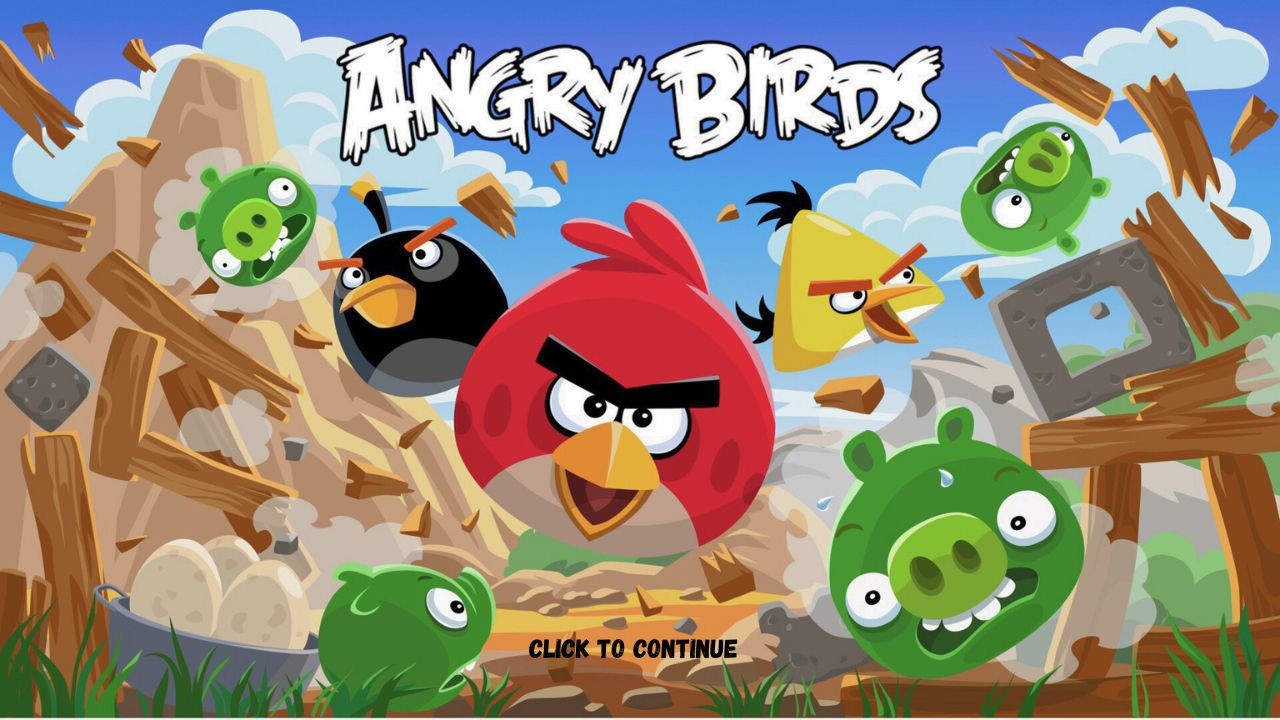
\includegraphics[width=0.5\textwidth]{assets/background-images/Angry_birds_loading_background.jpg}
    \caption{Game intro screen}
    \label{fig:game-intro}
\end{figure}

Tap anywhere in the image to continue to the Main Menu screen.


\subsubsection{Main Menu}
The main menu screen pops up as soon you left click on the game screen. Here you got three choices: Play game, Instructions, and settings.

\begin{figure}[h!]
    \centering
    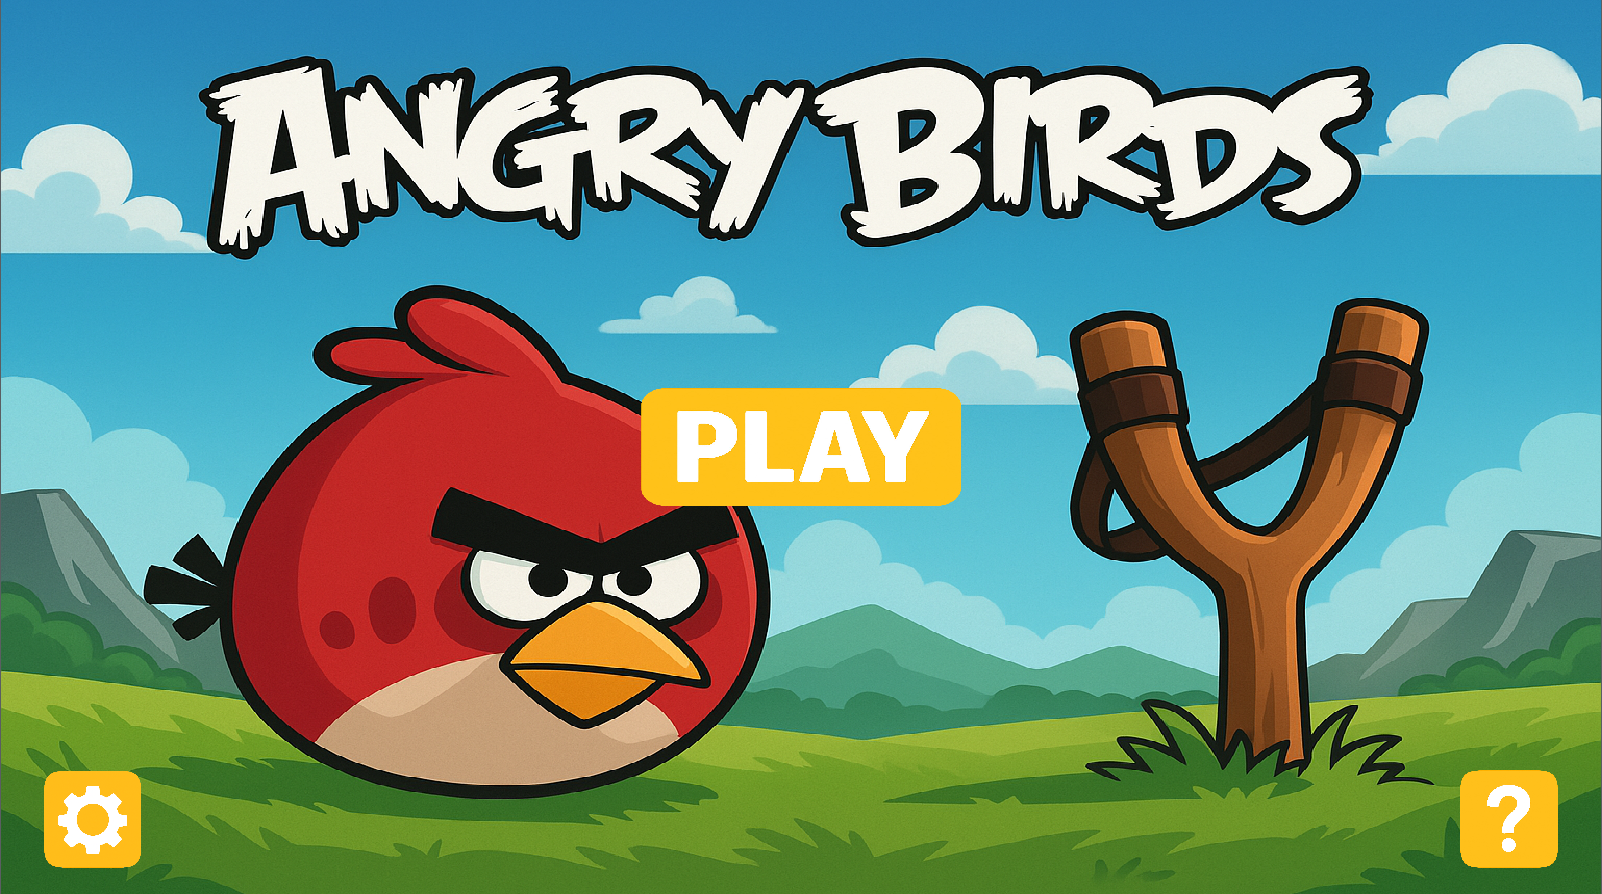
\includegraphics[width=0.5\textwidth]{assets/report_images/main_menu.png}
    \caption{Main Menu screen}
    \label{fig:main-menu}
\end{figure}

Tapping on play game will start the game, instructions will show you some basic instructions of the game and settings will let you toggle game sounds and game music on and off.


\subsubsection{Game level selection}
After you select play game, you will be taken to the level selection screen. Here you can select the level you want to play. The game has 3 levels, each with increasing difficulty. You can select the level by tapping on it.

\begin{figure}[h!]
    \centering
    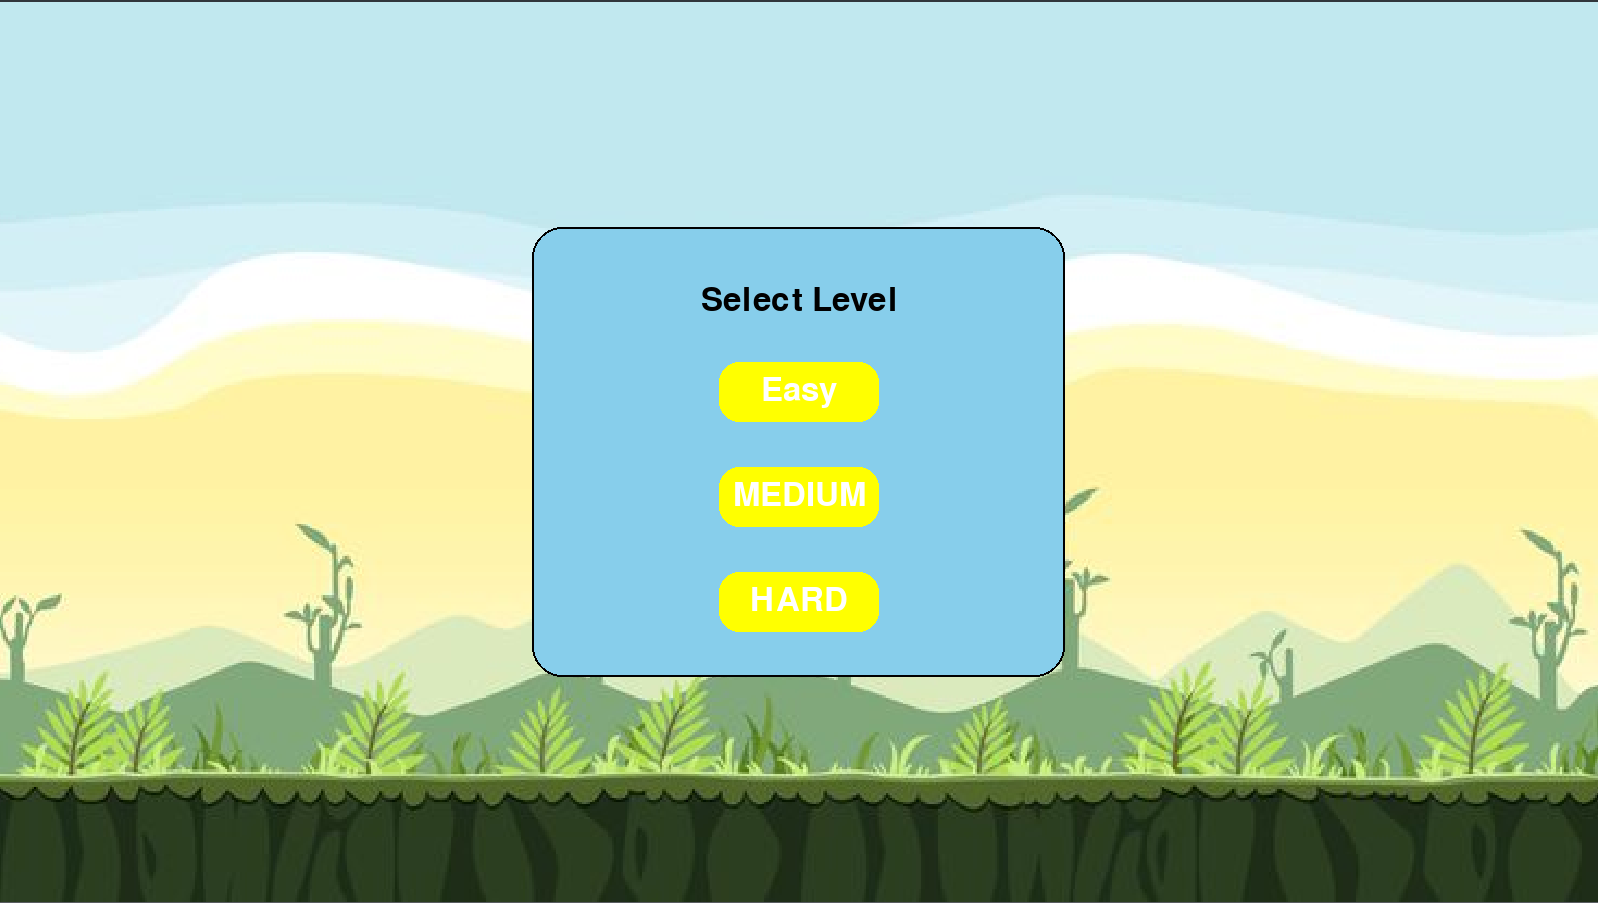
\includegraphics[width=0.5\textwidth]{assets/instruction-images/image0.png}
    \caption{Level selection screen}
    \label{fig:level-selection}
\end{figure}

All levels will have same bird abilities and same number of blocks(15 in total).
\begin{itemize}
    \item \textbf{Easy:} This level will be basic and nothing special
    \item \textbf{Medium:} This level will have wind mechanic, which will affect the bird's trajectory.
    \item \textbf{Hard:} This level will have wind mechanic, which will affect the bird's trajectory and also no path trajectory will be shown.
\end{itemize}


\subsubsection{Team selection}
After selecting the level, you will be taken to the team selection screen. 
Firstly, the first team input screen will pop up. Enter your name in the name field(can't be > 15) and then select the bird order you want by tapping on then sequentially.
The bird order will remain the same the whole game, and will act like a circular queue. There's a reset order button which will reset the order of the birds.

\begin{figure}[h!]
    \centering
    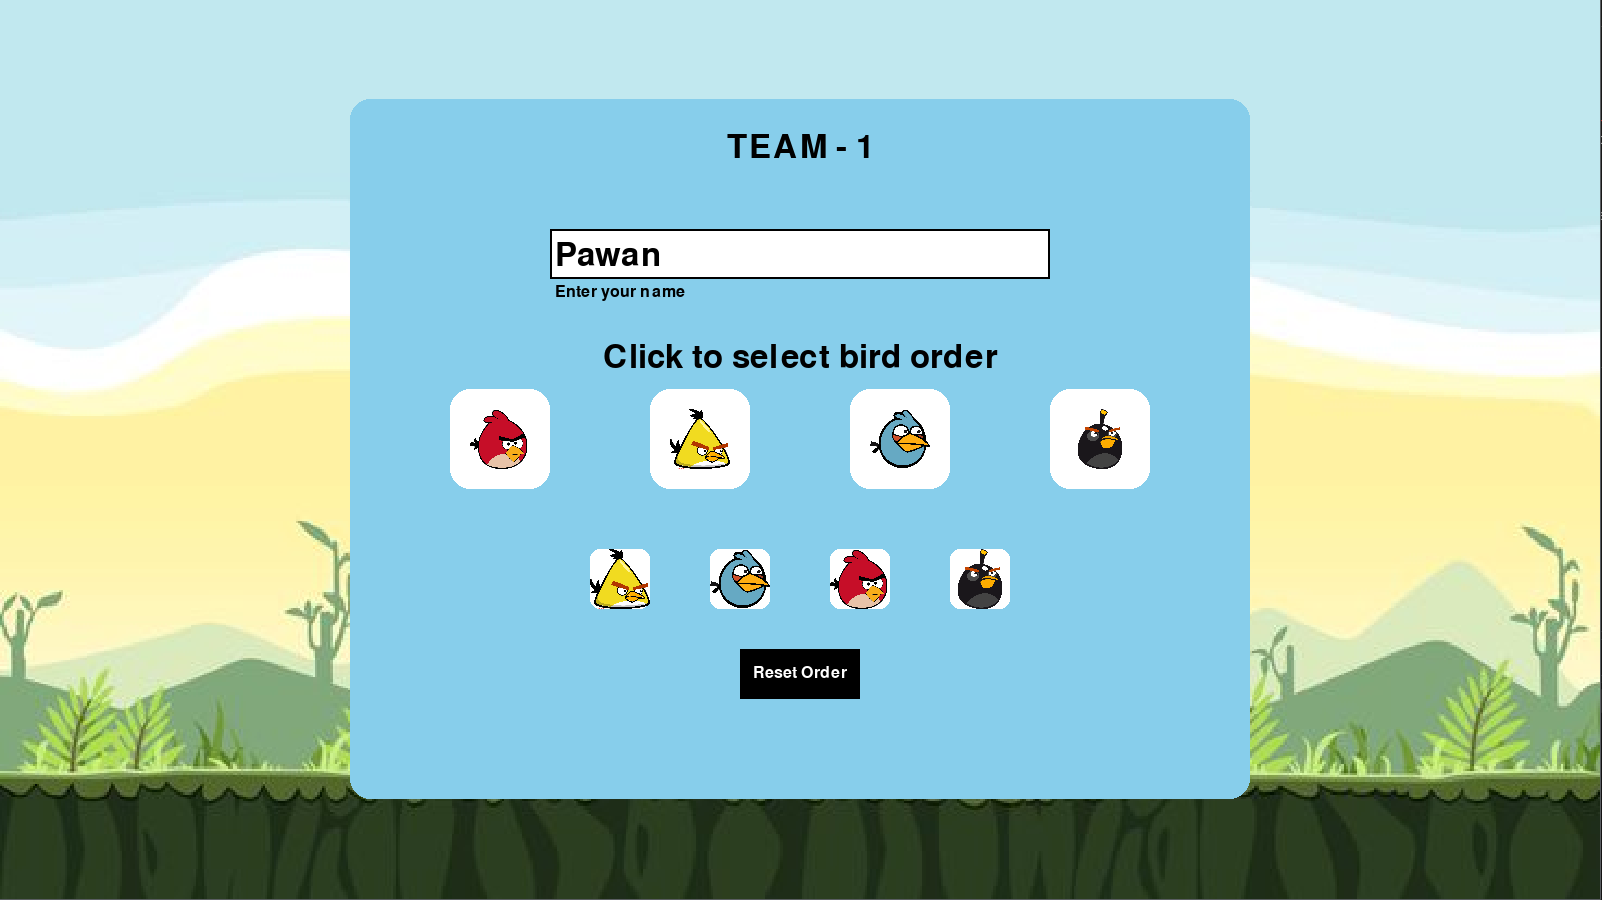
\includegraphics[width=0.5\textwidth]{assets/instruction-images/image1.png}
    \caption{Team selection screen}
    \label{fig:team-selection}
\end{figure}

When done, press the enter key and fill the seccond team info and then press enter key again and game will finally start!

\newpage
\subsubsection{Game screen}
The game screen will look like this:
\begin{figure}[h!]
    \centering
    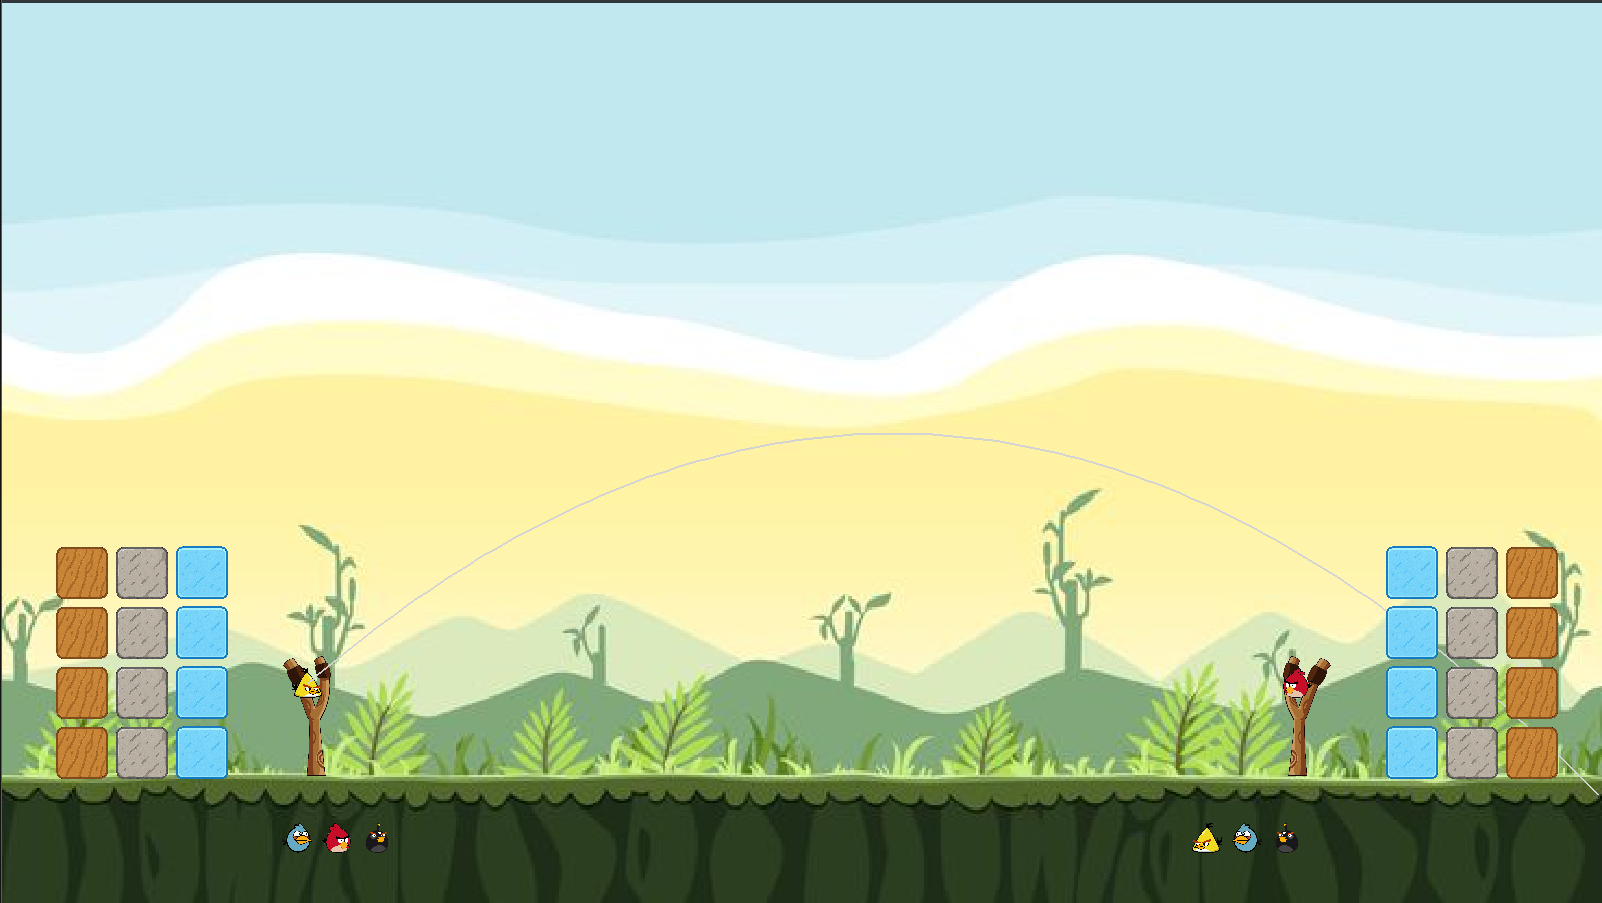
\includegraphics[width=0.5\textwidth]{assets/instruction-images/image2.png}
    \caption{Game screen}
    \label{fig:game-screen}
\end{figure}
Drag the slingshot to aim and release to launch the bird. The game will show you the trajectory of the bird, if you level is not hard. 
The game will show you the blocks remaining for both teams and also the velocity with which the bird is travelling.
On the top-right corner is a restart button, which takes you back to the level screen.


\subsubsection{Game end screen}
After all the blocks are destroyed, the game will show you the game end screen.
Here you can see the winner and also the time taken to complete the level. You can also restart the game from here.
\begin{figure}[h!]
    \centering
    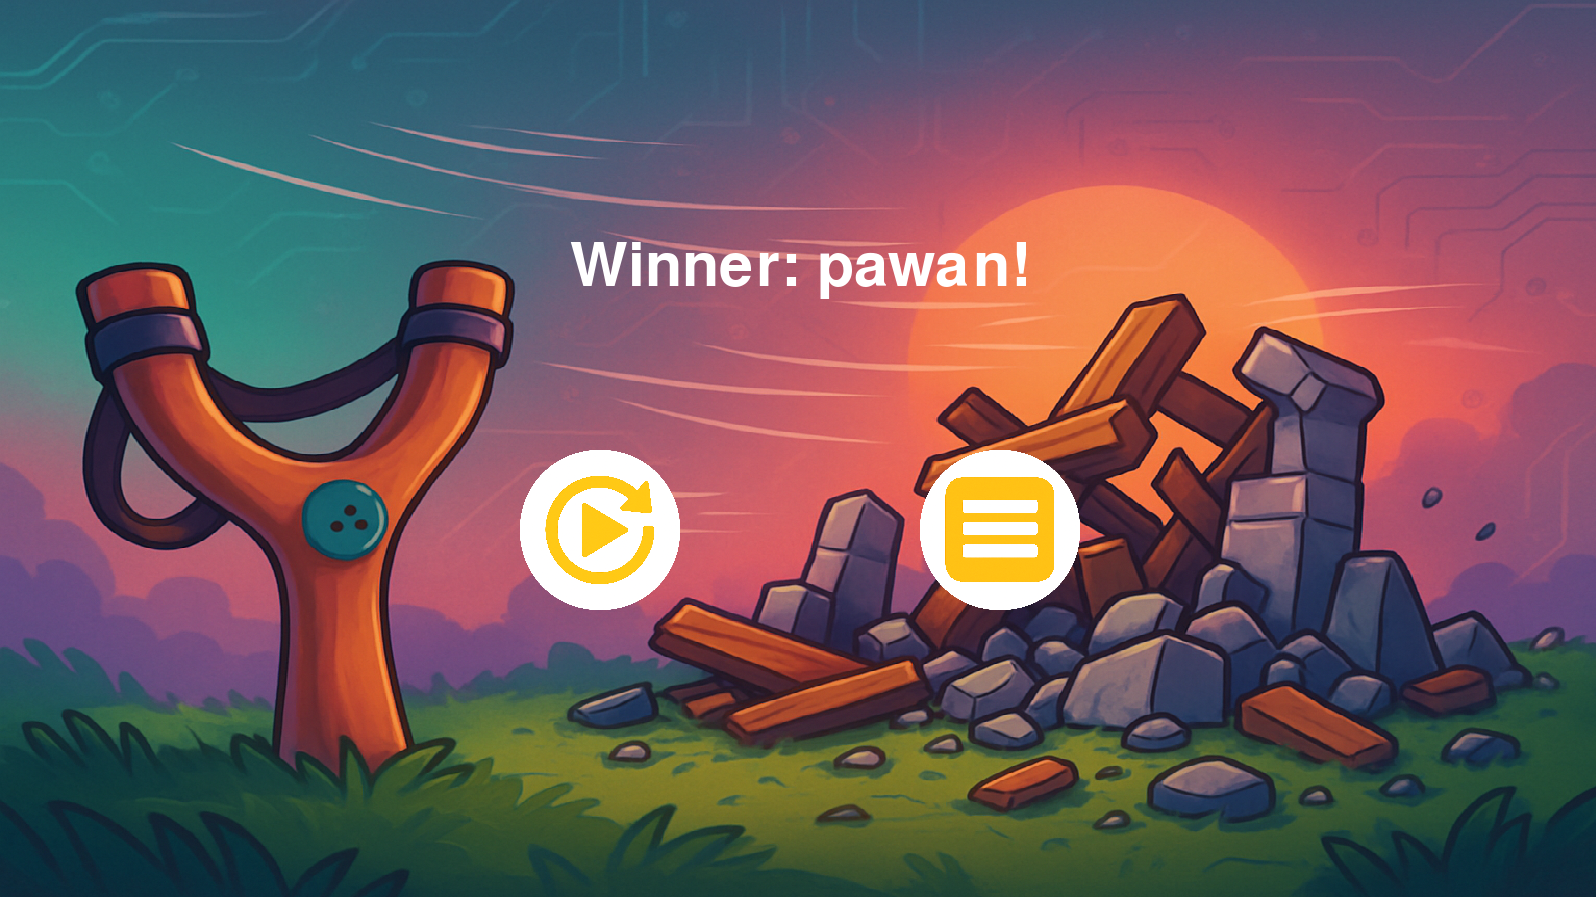
\includegraphics[width=0.5\textwidth]{assets/report_images/end_screen.png}
    \caption{Game end screen}
    \label{fig:game-end}
\end{figure}

Hit play again to start the game again with the same level and teams or you can hit the main menu button to go back to the main menu screen.


\subsection{Game Mechanics}\label{subsec:Game Mechanics}
\subsubsection{Birds}
The game has 4 types of birds, each with different abilities. The birds are:
\begin{itemize}
    \item \textbf{Red:} This is the basic bird, which has no special abilities. Deals same damage to all blocks.
    \item \textbf{Blues:} Deals 1.5x damage to ice block and 0.75 to wood and stone blocks
    \item \textbf{Chuck:} Deals 1.5x damage to wood blocks and 0.75x damage to stone and ice blocks.
    \item \textbf{Bomb:} First deals damage to the block dealing 1.25x damage to stone blocks, 0.5x damage to wood blocks and ice blocks and then explodes, dealing 0.3x damage to all blocks in the radius.
\end{itemize}

\subsubsection{Blocks}
The game has 3 types of blocks, each with different properties. The blocks are:
\begin{itemize}
    \item \textbf{Wood:} A block made of wood. Has 1500 hp
    \item \textbf{Ice:} A block made of ice. Has 2000 hp
    \item \textbf{Stone:} A block made of stone. Has 2500 hp
\end{itemize}

\subsubsection{Slingshot}
The slingshot is the main mechanic of the game. You can drag the slingshot ot aim and release the bird. 
The slingshot is clamped such that you can't shoot behind yourself. 
There's also a maximum pull, trying to pull beyond which won't increase the launch velocity.

\subsubsection{Damage}
The damage dealt by the birds depends on the velocity of the bird and the damage multiplier bird for the corresponding block type.

\begin{table}[h!]
    \centering
    \begin{tabular}{|c|c|c|c|c|}
        \hline
                       & \textbf{Red} & \textbf{Blues} & \textbf{Chuck} & \textbf{Bomb} \\ \hline
        \textbf{Wood}  & 1x           & 0.75x          & 1.5x           & 0.5x          \\ \hline
        \textbf{Ice}   & 1x           & 1.5x           & 0.75x          & 0.5x          \\ \hline
        \textbf{Stone} & 1x           & 0.75x          & 0.75x          & 1.25x         \\ \hline
    \end{tabular}
    \caption{Damage multipliers for different birds and block types}
    \label{tab:damage-multipliers}
\end{table}

\subsubsection{Motion factors}
The game uses a simple physics engine to calculate the motion of the birds. The motion factors are:
\begin{itemize}
    \item \textbf{Gravity:} The game uses a constant gravity.
    \item \textbf{Friction:} The game doesn't has fricton when the bird is first shoot and the friction comes to act when the bird first touches the ground. 
    If the bird is going in the opposite direction, with respect to the boxes, the friction is increased so as to complete the motion quickly as the remaining motion is useless.
    \item \textbf{Wind:} The game uses a constant wind speed in the medium and hard levels, the direction being opposite direction to the player's target.
\end{itemize}

\vspace{2cm}

\label{sec:References}
\begin{thebibliography}{9}
    \bibitem{pygameCEDoc}
    Pygame CE Official Documentation \url{https://pyga.me/docs/}.

    \bibitem{stackoverflow}
    Stackoverflow for help in implementations \url{https://stackoverflow.com/}.

    \bibitem{ChatGPT}
    ChatGPT, OpenAI for learning \url{https://chat.openai.com/}.

\end{thebibliography}

\end{document}


